\documentclass[10pt,twocolumn]{article}
\usepackage[margin=1.5 cm]{geometry}
\setlength{\columnsep}{0.6 cm}

\usepackage[]{graphicx}
\usepackage[skip=10pt,font=scriptsize]{caption}

\usepackage[usenames, dvipsnames]{color}

\usepackage{amsmath}
\usepackage{amssymb}

\begin{document}

\subsection*{Cryogenic temperatures}

Time until creation of first contaminant atom is [300]

\begin{displaymath}
\tau = \frac{\tau_s}{bN_0} = \frac{4\delta^2}{\Omega^2}\frac{\tau_{\text{eff}}}{bN_0},
\end{displaymath}

\noindent
where $b$ is the branching ratio to contaminant states and $N_0$ is the total number of atoms. Using the estimates from [302] and the quasiclassical formulas in [303] we calculate how \textit{b}, $\tau_{\text{eff}}$ \textit{and their relevant combinations} depend on the \textit{ambient} temperature.

Figure 1 indicates how the branching ratio decreases when the temperature is reduced from 300 K to 1 K. It goes down by about 1 order of magnitude for temperatures between 10 K and 30 K, and about 2 orders of magnitude for T between 1 and 5 K. (At 77 K the branching ratio is roughly 2-4 times smaller).

\begin{figure}[!h]
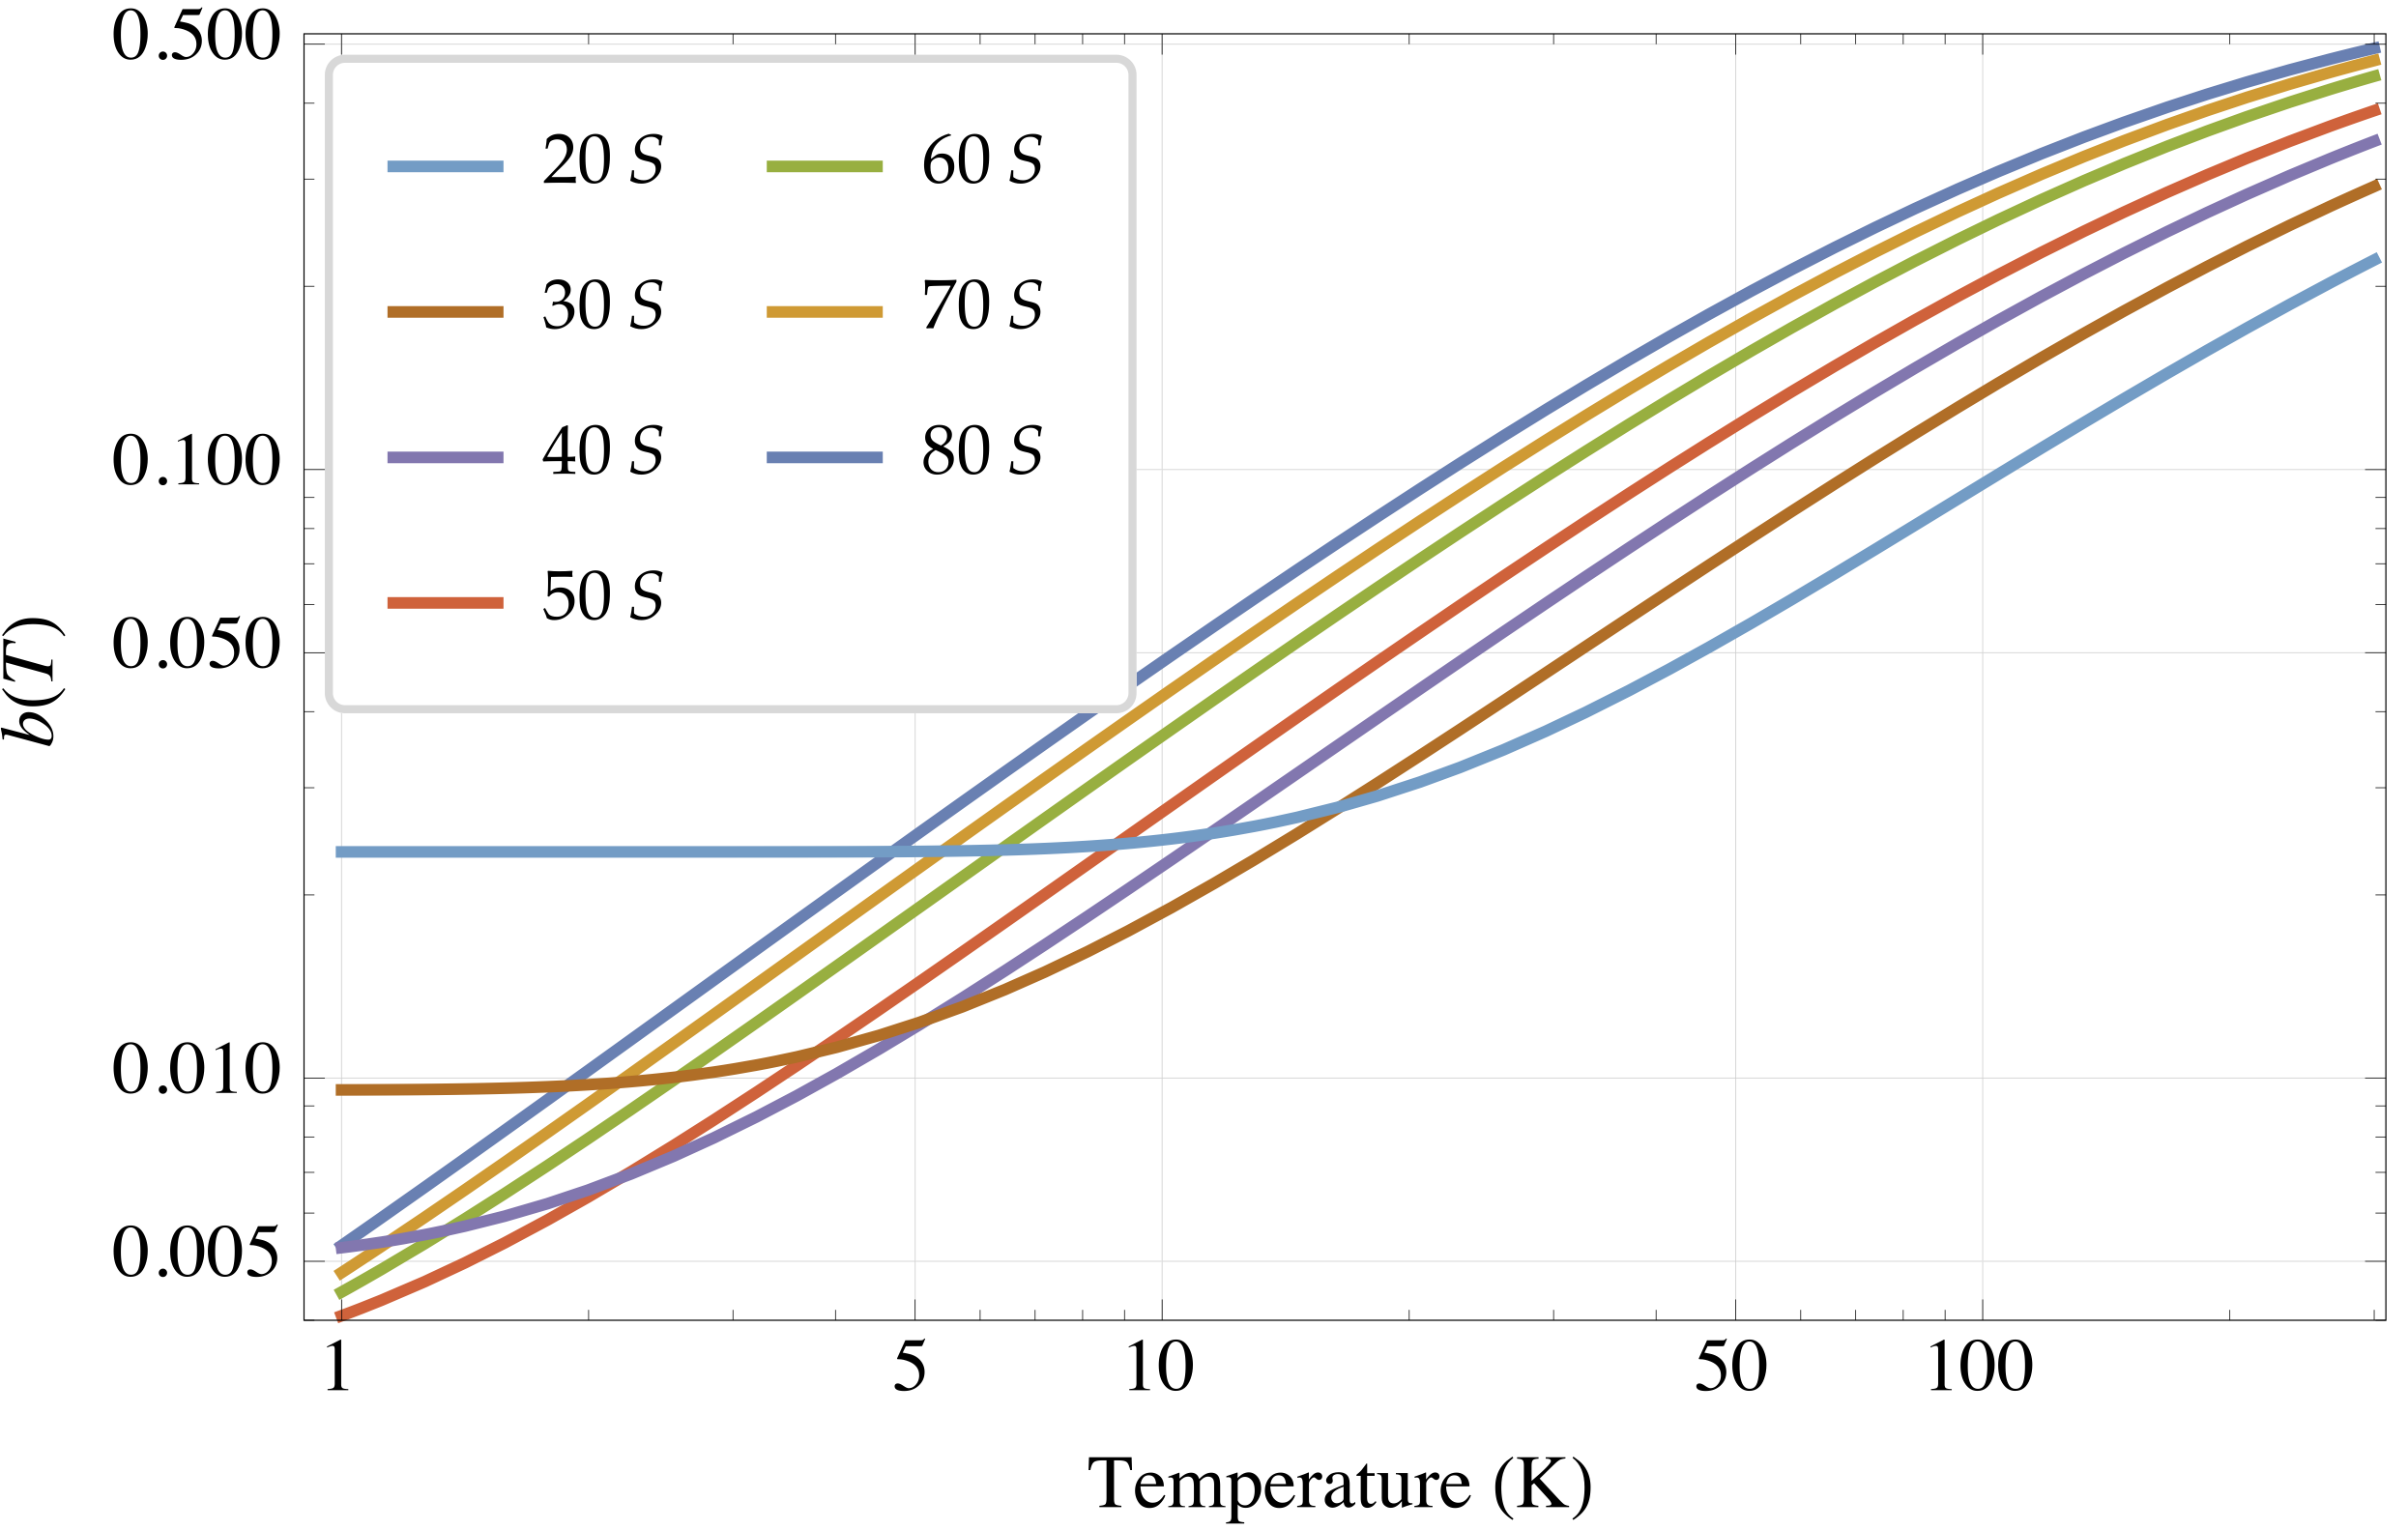
\includegraphics[scale=0.75]{bloglog.png} \caption{$b(T)$ vs $T$ for different $nS$ levels of $^{87}$Rb.}
\end{figure}

In figure 2 the

\begin{figure}[!h]
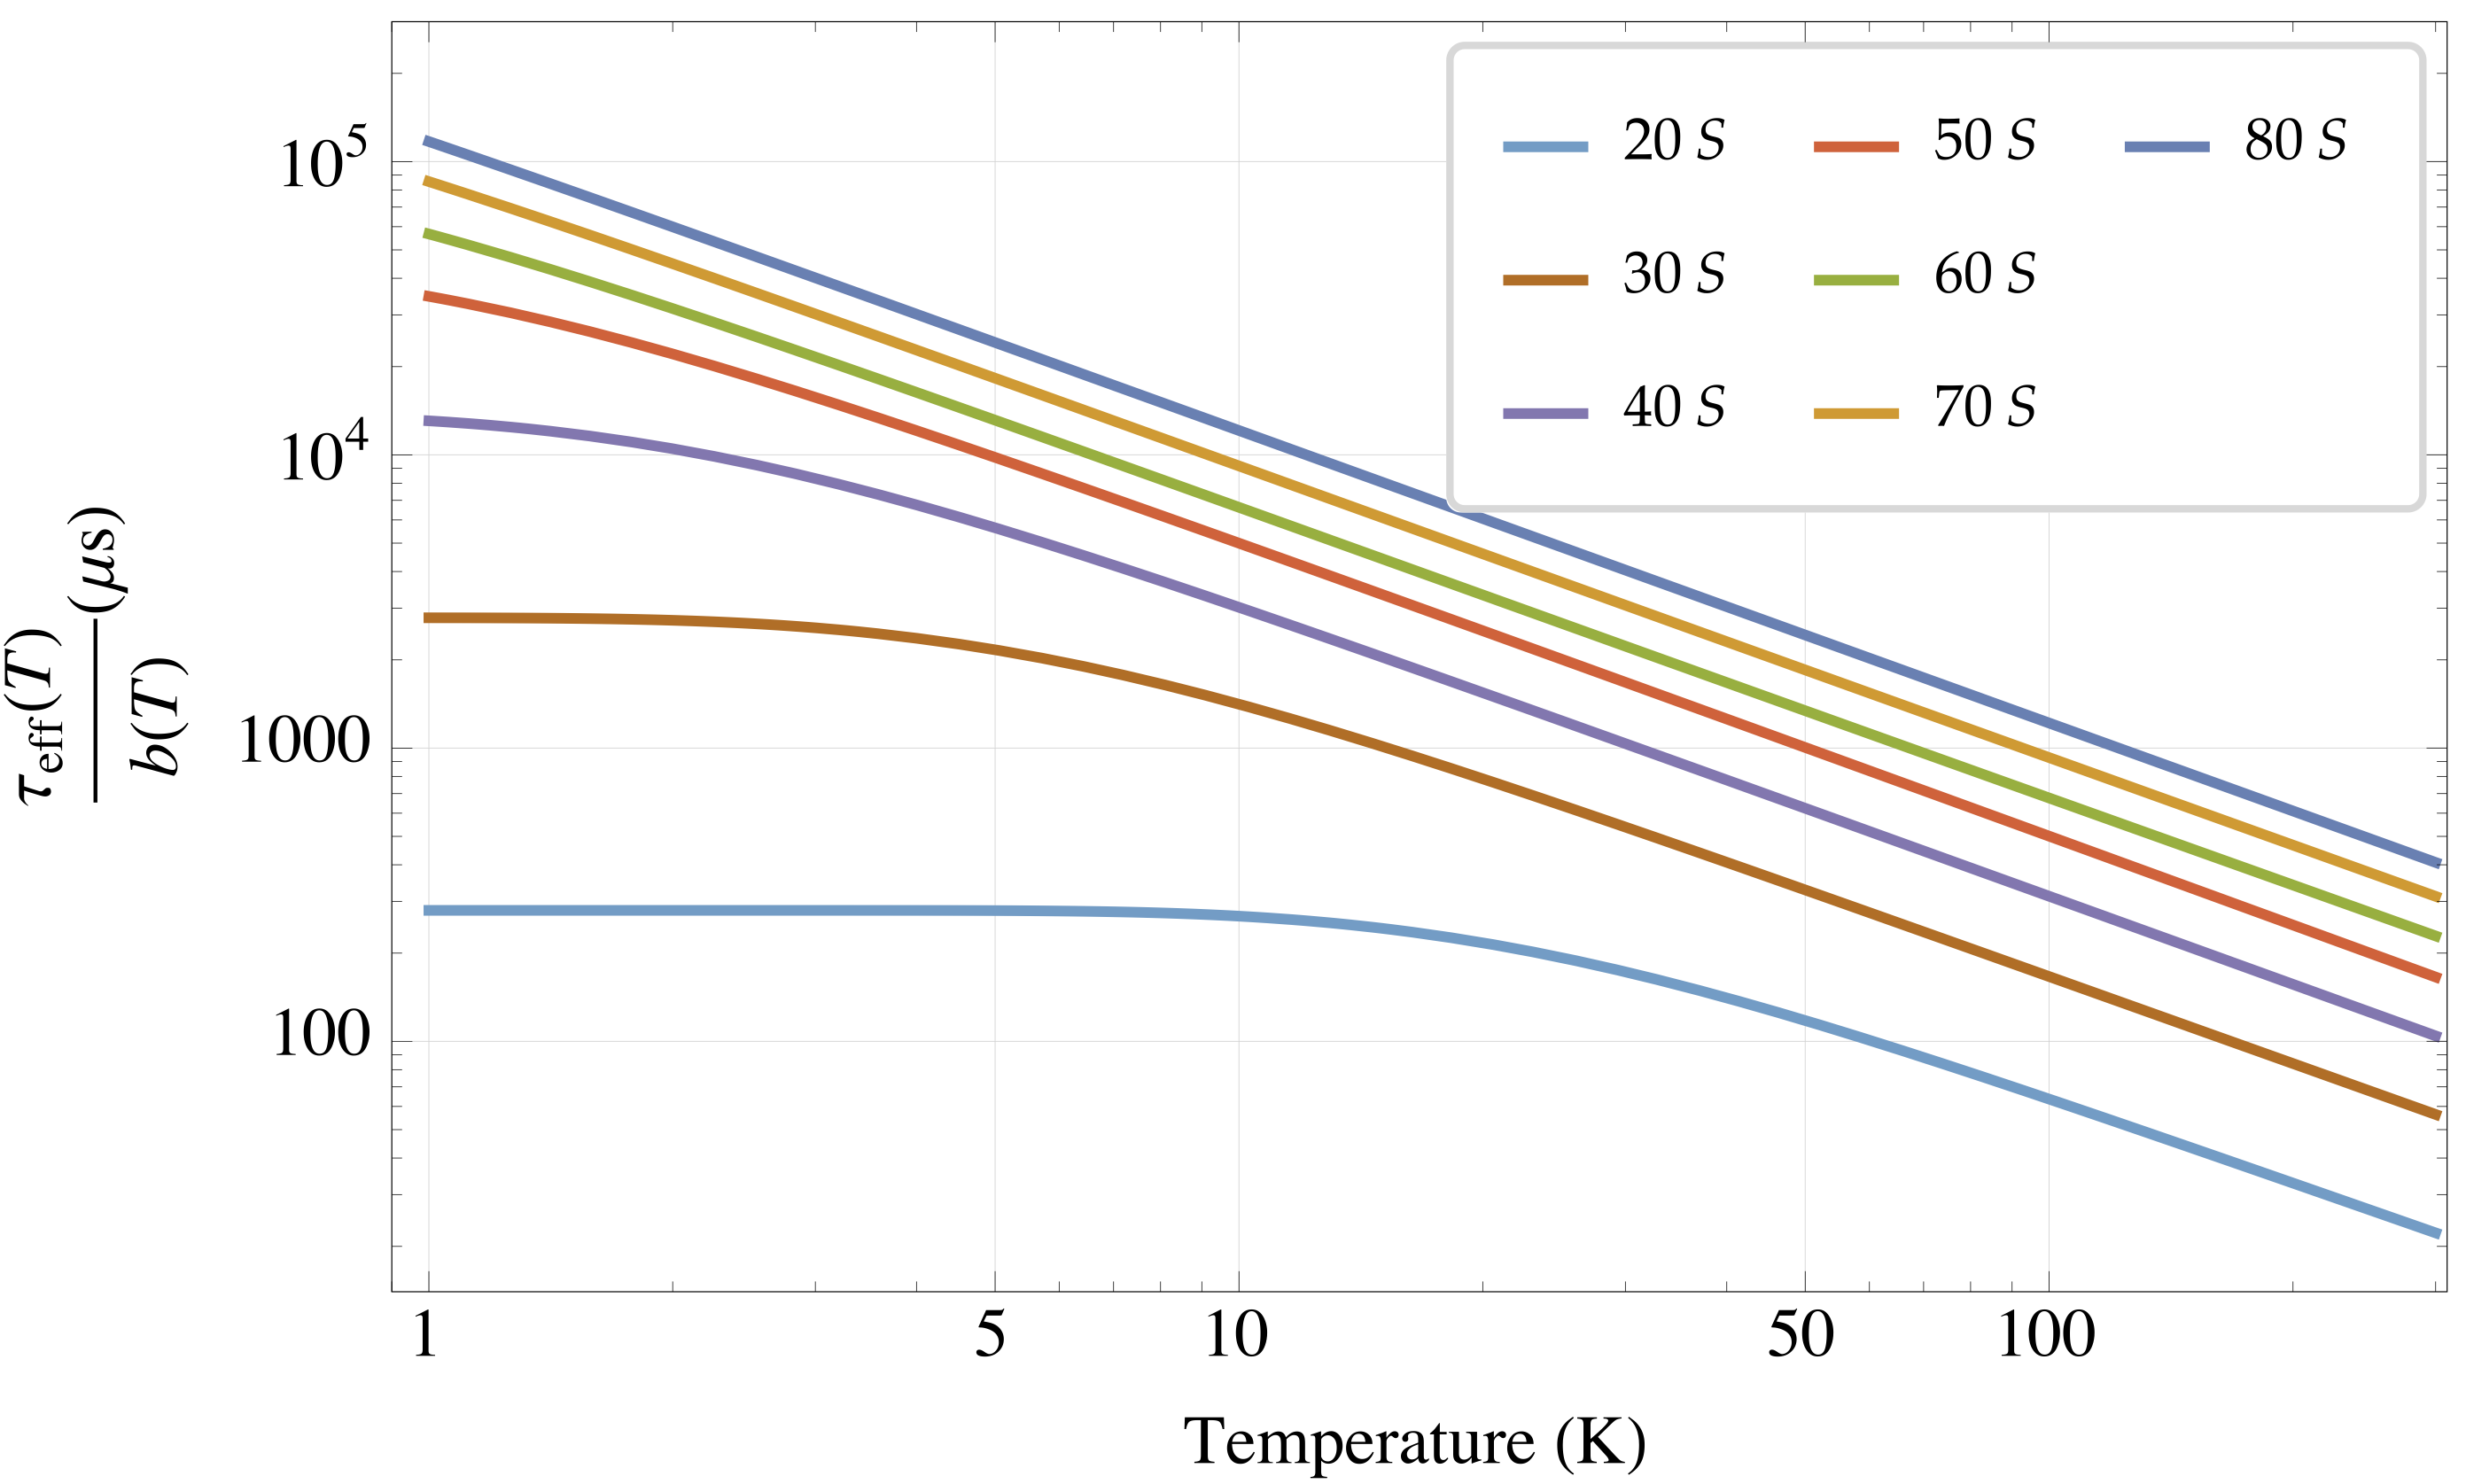
\includegraphics[scale=0.675]{tbloglog.png} \caption{$\frac{\tau_{\text{eff}}(T)}{b(T)}$ vs $T$ for different $nS$ levels of $^{87}$Rb.}
\end{figure}

Figure 3 shows the \textit{coherence} time reduction due to AB (proportional to $N^{-1}$) can only be \textit{fully} compensated for atom number less than

\begin{itemize}
\item 600 for $T\gtrsim 1$ K.
\item 100 for $T\gtrsim 5$ K.
\item 15 for $T\gtrsim 50$ K.
\end{itemize}
 
 From 1 K to 5 K one can \textit{expect to fully neutralize} the AB effect for a system between 100 and 500 atoms. From 50K to 100 K this would occur only with less than 15 atoms.
 
\begin{figure}[!h]
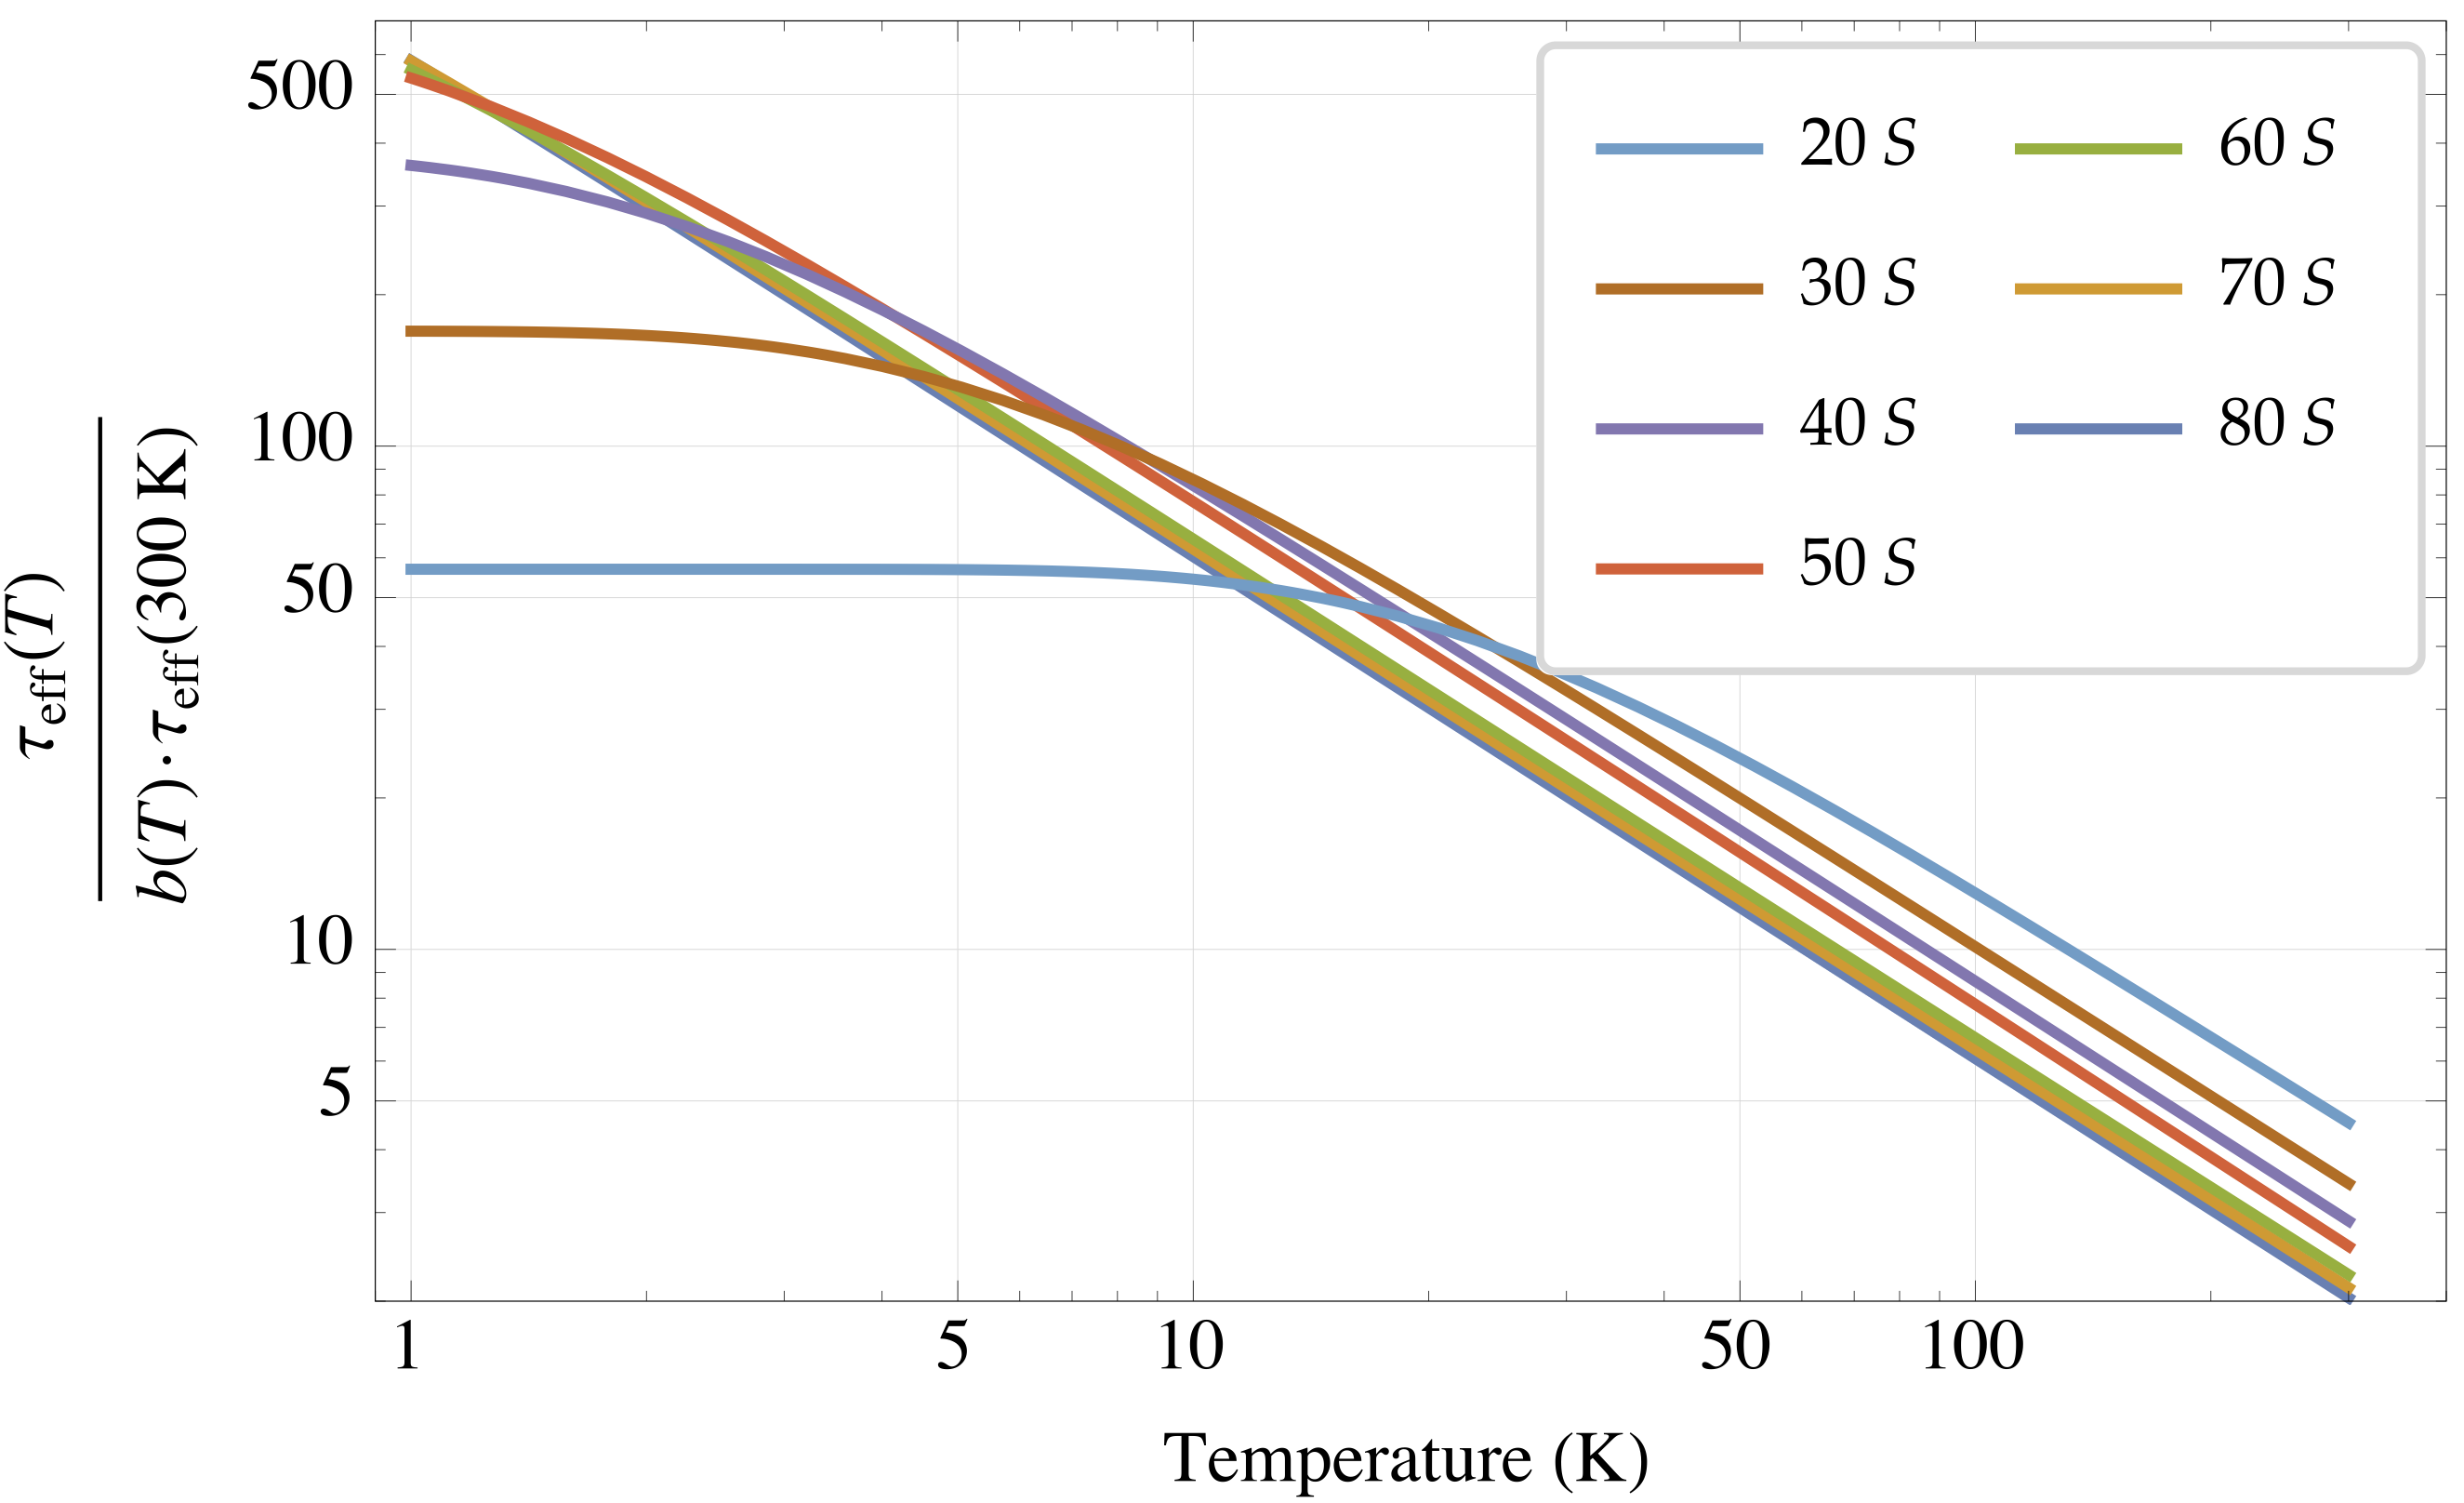
\includegraphics[scale=0.7]{tbtloglog.png} \caption{$\frac{\tau_{\text{eff}}(T)}{\tau_{\text{eff}}(300 \text{K})}\cdot\frac{1}{b(T)}$ vs $T$ for different $nS$ levels of $^{87}$Rb. \textit{The y axis can be interpreted as the atom number at which the $\frac{\tau_{\text{eff}}}{bN_0}$ factor becomes larger than $\tau_{\text{eff}}(300 K)$.}}
\end{figure}

\textit{How would this help certain proposals?} \ldots

\begin{itemize}
\item Reference [304, Pupillo] proposes a $N \lesssim 40$ atoms system to observe supersolid phases (\textcolor{ForestGreen}{This 2D system is purely repulsive, which makes me doubt is worth considering.}). The AB effect would be compensated for temperatures arond 20 K.
\item Ref [305, Glaetzle] proposes ealizing quantum spin ice in two dimensions using $16 \leq N_0\leq 72$. Reducing the black-body radiation temperature between 50 K and 10 K would make up for the AB decoherence effect.
\item \textcolor{ForestGreen}{Bloch Paper} using 200 atoms would require temperatures between 3 K and 5 K. (\textcolor{ForestGreen}{Not entirely sure since I need to check the vdW radius}).
\end{itemize}



\begin{center}
\rule{4cm}{0.4pt}
\end{center}

\begin{thebibliography}{8}
\bibitem{ABp} 
AB paper.
 
\bibitem{Beterov} 
I. I. Beterov, I. I. Ryabtsev, D. B. Tretyakov, and V. M. Entin,
Phys. Rev. A 79, 052504 (2009).

\bibitem{Dyachkov}
L. G. Dyachkov and P. M. Pankratov, J. Phys. B 27, 461
(1994).

\bibitem{PupilloZollerSS} G. Pupillo, A. Micheli, M. Boninsegni, I. Lesanovsky, and
P. Zoller, Phys. Rev. Lett. 104, 223002 (2010).

\bibitem{Spin-Ice}  A. W. Glaetzle, M. Dalmonte, R. Nath, C. Gross, I. Bloch, and P. Zoller, Phys. Rev. Lett. 114, 173002 (2015).

\bibitem{}
 
\end{thebibliography}

\end{document}